%-----------------------------------------------------------------------------%
\chapter{Metodologi Penelitian} \label{ch:metodologi}
%-----------------------------------------------------------------------------%

%-----------------------------------------------------------------------------%
\section{Desain Penelitian}
%-----------------------------------------------------------------------------%

Penelitian ini mengadopsi pendekatan eksperimental kuantitatif dengan metodologi \textit{comparative analysis} untuk mengevaluasi efektivitas \textit{ensemble weighted averaging} dalam deteksi \textit{deepfake}. Kerangka penelitian dirancang untuk membandingkan secara sistematis performa model \textit{deep learning} individual dengan pendekatan \textit{ensemble}, menggunakan metrik evaluasi komprehensif pada \textit{dataset} terstandarisasi.

\subsection{Alur Penelitian}

Untuk memberikan gambaran menyeluruh tentang metodologi yang diterapkan, Gambar~\ref{fig:research_methodology} menyajikan kerangka kerja penelitian secara konseptual, mulai dari persiapan data hingga analisis interpretasi.

\begin{figure}[H]
    \centering
    \fbox{\includegraphics[width=0.85\textwidth]{assets/pics/alur-besar.png}}
    \caption{Pipeline penelitian deepfake}
    \label{fig:research_methodology}
\end{figure}

Seperti yang terlihat pada Gambar~\ref{fig:research_methodology}, metodologi penelitian mengikuti alur sistematis yang dimulai dengan persiapan data, dilanjutkan dengan pengembangan model individual dalam empat arsitektur berbeda, penghitungan bobot ensemble berdasarkan validation accuracy, implementasi weighted averaging, dan diakhiri dengan evaluasi komprehensif melalui pengujian internal maupun cross-dataset untuk analisis komplementaritas dan performa individual.

\subsection{Kerangka Penelitian}

Untuk mencapai tujuan tersebut, metodologi penelitian disusun dalam lima tahapan utama yang berurutan, sebagaimana diuraikan di bawah ini:
\begin{enumerate}
    \item \textbf{Persiapan Data}: Meliputi akuisisi, \textit{preprocessing}, dan partisi \textit{dataset} untuk memastikan data siap digunakan dalam pelatihan dan evaluasi.
    \item \textbf{Pengembangan Model Individual}: Merancang, melatih, dan mengevaluasi empat arsitektur \textit{deep learning} yang berbeda untuk menciptakan keragaman dalam \textit{ensemble}.
    \item \textbf{Implementasi \textit{Ensemble}}: Mengembangkan model \textit{ensemble weighted averaging} dengan menghitung bobot berdasarkan performa validasi dari setiap model individual.
    \item \textbf{Evaluasi Komparatif}: Melakukan perbandingan sistematis antara performa model individual dengan model \textit{ensemble} menggunakan \textit{dataset} pengujian.
    \item \textbf{Analisis dan Interpretasi}: Menganalisis hasil secara statistik untuk menarik kesimpulan mengenai efektivitas pendekatan \textit{ensemble} dan implikasi praktisnya.
\end{enumerate}

\subsection{Desain Eksperimen}

Penelitian ini menggunakan desain eksperimen terkendali untuk mengukur pengaruh arsitektur model terhadap performa deteksi. Variabel-variabel dalam penelitian ini didefinisikan sebagai berikut:
\begin{itemize}
    \item \textbf{Variabel Bebas}: Arsitektur model yang digunakan, yaitu \textit{CNN}, \textit{ResNet50}, \textit{Xception}, dan \textit{EfficientNet-B4}.
    \item \textbf{Variabel Terikat}: Metrik performa yang diukur, meliputi \textit{Accuracy}, \textit{Precision}, \textit{Recall}, \textit{F1-Score}.
    \item \textbf{Variabel Terkendali}: Faktor-faktor yang dijaga konstan untuk memastikan validitas perbandingan, seperti \textit{dataset}, pipa \textit{preprocessing}, parameter pelatihan utama, dan metodologi evaluasi.
\end{itemize}

Validitas internal dijaga melalui prosedur standarisasi yang ketat pada seluruh tahapan eksperimen. Sementara itu, validitas eksternal ditingkatkan dengan menggunakan \textit{dataset} publik yang representatif dan metodologi yang dapat direplikasi.

%-----------------------------------------------------------------------------%
\section{Dataset dan Preprocessing}
%-----------------------------------------------------------------------------%

Pemilihan dan persiapan \textit{dataset} merupakan fondasi krusial dalam penelitian ini. Tahapan ini bertujuan untuk menyediakan data yang berkualitas, seimbang, dan relevan untuk melatih serta mengevaluasi model deteksi \textit{deepfake}.

\subsection{Karakteristik Dataset}

Penelitian ini menggunakan \textit{dataset} "140k Real and Fake Faces" yang diperoleh dari repositori \textit{Kaggle}. \textit{Dataset} ini dipilih karena relevansinya dengan tugas deteksi wajah asli versus palsu dan skalanya yang besar. Karakteristik utama dari \textit{dataset} ini dirangkum dalam Tabel \ref{tab:dataset_characteristics}.

\begin{table}[H]
\centering
\caption{Karakteristik data "140k Real and Fake Faces"}
\label{tab:dataset_characteristics}
\begin{tabular}{|l|l|}
\hline
\textbf{Karakteristik} & \textbf{Spesifikasi} \\
\hline
Total Gambar & 140.000 \\
Gambar Asli (\textit{Real}) & 70.000 (50\%) \\
Gambar Palsu (\textit{Fake}) & 70.000 (50\%) \\
Format Gambar & JPEG \\
Resolusi & 256 × 256 piksel \\
\textit{Color Space} & RGB \\
Sumber Gambar Asli & \textit{Flickr} (Koleksi \textit{Nvidia}) \\
Sumber Gambar Palsu & \textit{StyleGAN Generated} \\
\hline
\end{tabular}
\end{table}

\subsection{Partisi Dataset}

Untuk memastikan evaluasi yang objektif, \textit{dataset} dibagi menjadi tiga subset: pelatihan, validasi, dan pengujian. Pembagian ini menggunakan teknik \textit{stratified sampling} untuk menjaga distribusi kelas yang seimbang pada setiap subset. Proporsi pembagiannya adalah sebagai berikut:

\begin{align}
D_{train} &= 100.000 \text{ gambar (71.4\%)} \\
D_{val} &= 20.000 \text{ gambar (14.3\%)} \\
D_{test} &= 20.000 \text{ gambar (14.3\%)}
\end{align}

\subsection{Pipa Preprocessing}

Pipa \textit{preprocessing} diimplementasikan menggunakan generator data dari framework deep learning. Proses ini mencakup normalisasi nilai piksel dan augmentasi data. Konfigurasi yang berbeda diterapkan untuk data pelatihan dan data evaluasi (validasi dan pengujian).

\subsubsection{Preprocessing Data Pelatihan}

Generator data pelatihan dikonfigurasi dengan berbagai parameter untuk mengoptimalkan proses pembelajaran. Pertama, dilakukan normalisasi piksel dengan membagi setiap nilai piksel dengan 255 untuk mengubah skala dari rentang 0-255 menjadi 0-1, yang membantu stabilitas proses pelatihan. Augmentasi data berupa \textit{horizontal flip} diterapkan secara acak pada gambar untuk meningkatkan variasi data dan mencegah overfitting. Ukuran target gambar ditetapkan pada 256×256 piksel untuk konsistensi dengan arsitektur model. Batch size diatur pada 32 untuk keseimbangan antara efisiensi komputasi dan penggunaan memori. Mode kelas ditetapkan sebagai binary karena ini adalah masalah klasifikasi dua kelas (real vs fake). Terakhir, shuffle diaktifkan untuk memastikan urutan data acak pada setiap epoch, yang membantu proses konvergensi model.

\subsubsection{Preprocessing Data Validasi dan Pengujian}

Untuk data validasi dan pengujian, konfigurasi generator dibuat lebih sederhana dan deterministik. Normalisasi piksel tetap diterapkan dengan cara yang sama seperti data pelatihan untuk konsistensi. Namun, tidak ada augmentasi data yang diterapkan untuk memastikan evaluasi dilakukan pada data orisinal yang tidak dimodifikasi. Ukuran target gambar tetap 256×256 piksel untuk konsistensi. Untuk data validasi, batch size diatur pada 16 untuk efisiensi proses evaluasi, sedangkan untuk data pengujian menggunakan batch size 1 untuk prediksi individual yang lebih presisi. Mode kelas tetap binary, dan shuffle dinonaktifkan untuk mempertahankan urutan data asli selama evaluasi.

\subsection{Strategi Augmentasi Data}

Strategi augmentasi data secara sengaja dibatasi hanya pada \textit{horizontal flipping} untuk \textit{set} pelatihan. Keputusan ini didasarkan pada pertimbangan berikut:
\begin{itemize}
    \item \textbf{Preservasi Artefak}: Menghindari augmentasi yang lebih agresif (seperti rotasi, \textit{zoom}, atau \textit{shear}) yang berpotensi menghilangkan atau merusak artefak kompresi halus yang sering menjadi penanda utama citra \textit{deepfake}.
    \item \textbf{Integritas Spasial}: Mempertahankan hubungan spasial fitur wajah yang penting untuk proses deteksi.
    \item \textbf{Efisiensi Komputasi}: Menjaga proses pelatihan agar tetap efisien secara komputasi.
\end{itemize}
Contoh visual dari penerapan augmentasi sederhana ini disajikan pada Gambar \ref{fig:augmentation_simple}, yang menunjukkan perbandingan gambar sebelum dan sesudah operasi \textit{horizontal flip}.

\begin{figure}[h]
\centering
% Menambahkan \fbox{} untuk membuat bingkai di sekitar gambar
\fbox{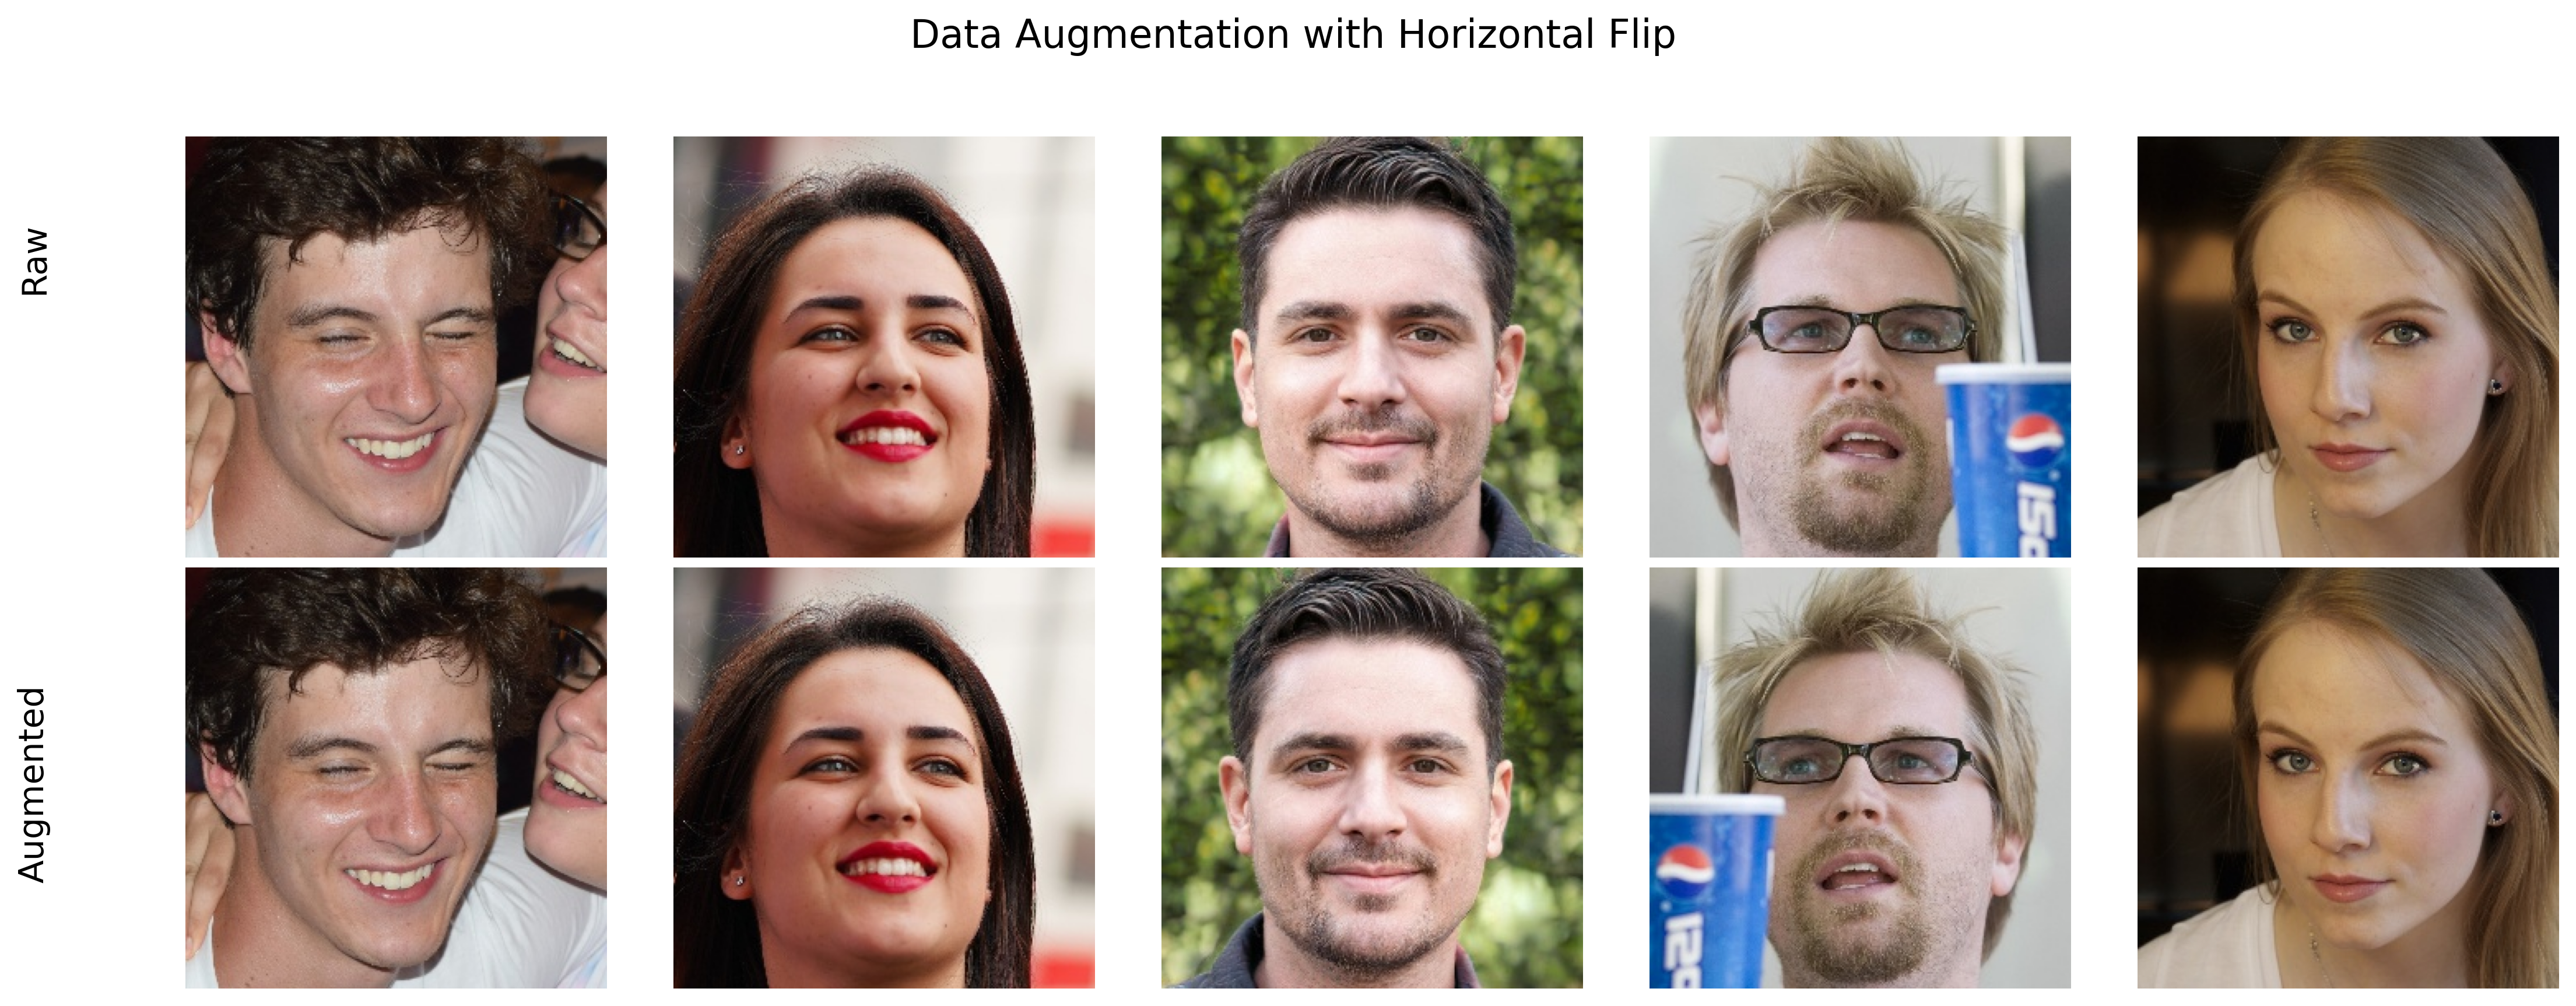
\includegraphics[width=0.8\textwidth]{assets/pics/augmentation_simple.png}}
\caption{Perbandingan gambar sebelum dan sesudah augmentasi sederhana (\textit{horizontal flip})}
\label{fig:augmentation_simple}
\end{figure}

%-----------------------------------------------------------------------------%
\section{Arsitektur Model Individual}
%-----------------------------------------------------------------------------%

Penelitian ini mengimplementasikan empat arsitektur \textit{deep learning} yang dipilih untuk memberikan keragaman pada model ansambel. Setiap model memiliki karakteristik komplementer, mulai dari arsitektur sederhana yang dirancang khusus hingga model \textit{state-of-the-art} yang memanfaatkan \textit{transfer learning}.

\subsection{Arsitektur Custom CNN}

Sebuah \textit{Convolutional Neural Network (CNN)} dirancang dengan arsitektur hierarkis yang memanfaatkan karakteristik CNN dalam ekstraksi fitur lokal-ke-global, dengan harapan dapat mendeteksi inkonsistensi yang umum pada citra \textit{deepfake}. Spesifikasi lengkap arsitektur disajikan pada Tabel \ref{tab:custom_cnn_arch}. Setiap blok konvolusi mengintegrasikan regularisasi \textit{Dropout} untuk mencegah \textit{overfitting}. Peningkatan jumlah \textit{filter} secara hierarkis (32 $\rightarrow$ 64 $\rightarrow$ 128 $\rightarrow$ 256) memungkinkan model untuk mempelajari fitur dari level rendah (tepi, tekstur) hingga level tinggi (pola wajah).

\begin{table}[H]
\centering
\caption{Arsitektur dari model CNN}
\label{tab:custom_cnn_arch}
\begin{tabular}{|l|l|l|l|}
\hline
\textbf{Jenis \textit{Layer}} & \textbf{\textit{Output Shape}} & \textbf{Konfigurasi} & \textbf{Aktivasi} \\
\hline
\textit{InputLayer} & (256, 256, 3) & - & - \\
\hline
\textit{Conv2D} & (256, 256, 32) & 32 \textit{filter}, 3×3 & \textit{ReLU} \\
\textit{Conv2D} & (256, 256, 32) & 32 \textit{filter}, 3×3 & \textit{ReLU} \\
\textit{MaxPooling2D} & (128, 128, 32) & 2×2 \textit{pool size} & - \\
\textit{Dropout} & (128, 128, 32) & \textit{rate}=0.25 & - \\
\hline
\textit{Conv2D} & (128, 128, 64) & 64 \textit{filter}, 3×3 & \textit{ReLU} \\
\textit{Conv2D} & (128, 128, 64) & 64 \textit{filter}, 3×3 & \textit{ReLU} \\
\textit{MaxPooling2D} & (64, 64, 64) & 2×2 \textit{pool size} & - \\
\textit{Dropout} & (64, 64, 64) & \textit{rate}=0.25 & - \\
\hline
\textit{Conv2D} & (64, 64, 128) & 128 \textit{filter}, 3×3 & \textit{ReLU} \\
\textit{Conv2D} & (64, 64, 128) & 128 \textit{filter}, 3×3 & \textit{ReLU} \\
\textit{MaxPooling2D} & (32, 32, 128) & 2×2 \textit{pool size} & - \\
\textit{Dropout} & (32, 32, 128) & \textit{rate}=0.25 & - \\
\hline
\textit{Conv2D} & (32, 32, 256) & 256 \textit{filter}, 3×3 & \textit{ReLU} \\
\textit{Conv2D} & (32, 32, 256) & 256 \textit{filter}, 3×3 & \textit{ReLU} \\
\textit{MaxPooling2D} & (16, 16, 256) & 2×2 \textit{pool size} & - \\
\textit{Dropout} & (16, 16, 256) & \textit{rate}=0.25 & - \\
\hline
\textit{Flatten} & (65536,) & - & - \\
\textit{Dense} & (512,) & \textit{L2 reg}=0.01 & \textit{ReLU} \\
\textit{BatchNormalization} & (512,) & - & - \\
\textit{Dropout} & (512,) & \textit{rate}=0.5 & - \\
\textit{Dense} & (128,) & \textit{L2 reg}=0.01 & \textit{ReLU} \\
\textit{BatchNormalization} & (128,) & - & - \\
\textit{Dropout} & (128,) & \textit{rate}=0.5 & - \\
\textit{Dense (Output)} & (1,) & - & \textit{Sigmoid} \\
\hline
\end{tabular}
\end{table}

\subsection{Arsitektur Transfer Learning}

Tiga model lainnya diimplementasikan menggunakan pendekatan \textit{transfer learning} dengan bobot \textit{pre-train} dari \textit{ImageNet}. Strategi \textit{fine-tuning} diterapkan pada semua model ini.

\subsubsection{ResNet50}
Model \textit{ResNet50} dipilih karena kemampuannya mengatasi masalah \textit{vanishing gradient} melalui \textit{residual connection}. Strategi \textit{fine-tuning} diterapkan dengan membekukan 100 \textit{layer} pertama untuk mempertahankan fitur umum tingkat rendah, sementara \textit{layer}-*\textit{layer}* berikutnya dilatih ulang untuk beradaptasi dengan domain deteksi \textit{deepfake}.

\subsubsection{Xception}
Arsitektur \textit{Xception} (Extreme Inception) memanfaatkan \textit{depthwise separable convolutions} untuk ekstraksi fitur yang efisien. Operasi ini memisahkan korelasi spasial dan \textit{cross-channel}, menjadikannya sangat efektif dalam menangkap inkonsistensi halus pada citra yang dimanipulasi secara digital seperti \textit{deepfake}.

\subsubsection{EfficientNet-B4}
\textit{EfficientNet-B4} dipilih karena pendekatan \textit{compound scaling} yang inovatif, yang secara seimbang menskalakan kedalaman (\textit{depth}), lebar (\textit{width}), dan resolusi jaringan. Hal ini menghasilkan keseimbangan optimal antara akurasi dan efisiensi komputasi, menjadikannya kandidat yang kuat untuk aplikasi praktis.

%-----------------------------------------------------------------------------%
\section{Metodologi Ensemble Weighted Averaging}
%-----------------------------------------------------------------------------%

Untuk meningkatkan robustisitas dan akurasi deteksi, prediksi dari keempat model individual digabungkan menggunakan metode \textit{ensemble weighted averaging}. Bagian ini menjelaskan dasar teoretis, strategi penentuan bobot, implementasi teknis, dan contoh perhitungan konkret dari pendekatan ini.

\subsection{Fondasi Teoretis}

\textit{Ensemble weighted averaging} beroperasi pada prinsip bahwa kombinasi linear dari beberapa model yang beragam, dengan bobot yang ditetapkan secara strategis, dapat menghasilkan prediksi yang lebih akurat dan stabil daripada prediksi model tunggal mana pun. Berdasarkan formulasi matematika yang telah dijelaskan dalam Bab 2 (Persamaan~\ref{eq:weighted_ensemble}).

\subsection{Strategi Perhitungan Bobot}

Bobot ($w_i$) untuk setiap model tidak ditetapkan secara seragam, melainkan dihitung berdasarkan performa masing-masing model pada \textit{dataset} validasi menggunakan formula yang telah didefinisikan dalam Persamaan~\ref{eq:performance_weight}. Pendekatan ini secara intuitif memberikan pengaruh yang lebih besar kepada model dengan performa validasi terbaik, sambil tetap mempertimbangkan kontribusi dari model lainnya.

\subsection{Contoh Perhitungan Bobot Ensemble}

Untuk memberikan pemahaman yang lebih konkret mengenai mekanisme perhitungan bobot, berikut disajikan contoh perhitungan menggunakan data hipotetis yang mudah dipahami:

\subsubsection{Skenario Contoh}
Misalkan kita memiliki empat model dengan validation accuracy sebagai berikut:
\begin{itemize}
    \item Model A (Custom CNN): 95,0\%
    \item Model B (ResNet50): 88,0\%
    \item Model C (Xception): 97,0\%
    \item Model D (EfficientNet): 92,0\%
\end{itemize}

\subsubsection{Langkah 1: Menghitung Total Validation Accuracy}
$$\text{Total} = 95,0 + 88,0 + 97,0 + 92,0 = 372,0$$

\subsubsection{Langkah 2: Menghitung Bobot Individual}
Menggunakan Persamaan~\ref{eq:performance_weight}:

\begin{align}
w_A &= \frac{95,0}{372,0} = 0,255 \text{ (25,5\%)} \\
w_B &= \frac{88,0}{372,0} = 0,237 \text{ (23,7\%)} \\
w_C &= \frac{97,0}{372,0} = 0,261 \text{ (26,1\%)} \\
w_D &= \frac{92,0}{372,0} = 0,247 \text{ (24,7\%)}
\end{align}

\subsubsection{Langkah 3: Verifikasi}
$$w_A + w_B + w_C + w_D = 0,255 + 0,237 + 0,261 + 0,247 = 1,000 \checkmark$$

\subsection{Mekanisme Prediksi Ensemble}

Setelah bobot diperoleh, prediksi ensemble untuk sebuah input $x$ dihitung sebagai berikut:

\subsubsection{Skenario Prediksi}
Misalkan untuk sebuah citra input, masing-masing model menghasilkan probabilitas:
\begin{itemize}
    \item Model A: 0,85 (85\% yakin citra adalah deepfake)
    \item Model B: 0,78 (78\% yakin citra adalah deepfake)
    \item Model C: 0,92 (92\% yakin citra adalah deepfake)
    \item Model D: 0,81 (81\% yakin citra adalah deepfake)
\end{itemize}

\subsubsection{Perhitungan Prediksi Ensemble}
Menggunakan Persamaan~\ref{eq:weighted_ensemble}:

\begin{align}
\hat{y}_{ensemble} &= (0,255 \times 0,85) + (0,237 \times 0,78) + (0,261 \times 0,92) + (0,247 \times 0,81) \\
&= 0,217 + 0,185 + 0,240 + 0,200 \\
&= 0,842
\end{align}

Hasil ini berarti model ensemble memiliki confidence 84,2\% bahwa citra tersebut adalah deepfake.

\subsection{Kerangka Implementasi}

Model \textit{ensemble} dibangun menggunakan API fungsional untuk menggabungkan beberapa model klasifikasi citra yang telah dilatih sebelumnya. Setiap model individual diperlakukan sebagai \textit{feature extractor} dan tidak diperbarui lagi selama proses inferensi dengan membekukan bobotnya.

Implementasi ansambel ini mengadopsi pendekatan \textit{weighted averaging}, di mana proses dimulai dengan pembuatan layer input yang konsisten untuk semua model dengan bentuk (256, 256, 3). Setiap model yang telah dilatih kemudian menerima input yang sama dan menghasilkan output probabilistik individual. Output dari masing-masing model kemudian dikalikan dengan bobot yang telah dihitung berdasarkan performa validasi mereka. Bobot ini mencerminkan kontribusi relatif setiap model terhadap prediksi akhir, dimana model dengan akurasi validasi yang lebih tinggi mendapat bobot yang lebih besar. Hasil perkalian antara output model dan bobotnya kemudian dijumlahkan untuk menghasilkan prediksi ensemble final. Seluruh proses ini diintegrasikan dalam satu model ensemble yang dapat melakukan inferensi secara end-to-end, mengambil input citra dan menghasilkan prediksi gabungan yang memanfaatkan kekuatan kolektif dari semua model individual.

%-----------------------------------------------------------------------------%
\section{Prosedur Pelatihan}
%-----------------------------------------------------------------------------%

Untuk memastikan perbandingan yang objektif dan valid antara model individual dan pendekatan \textit{ensemble}, penelitian ini menerapkan serangkaian prosedur pelatihan yang terstandarisasi. Bagian ini merinci protokol pelatihan yang digunakan, termasuk konfigurasi \textit{hyperparameter} dan \textit{callback}.

\subsection{Protokol Pelatihan}

Setiap model individual dilatih menggunakan protokol yang konsisten untuk menjamin keadilan dalam perbandingan. Perbedaan hanya terdapat pada \textit{learning rate} awal, yang disesuaikan berdasarkan karakteristik arsitektur (\textit{custom} vs. \textit{transfer learning}).

\subsubsection{Konfigurasi \textit{Hyperparameter}}
\textit{Hyperparameter} yang digunakan selama fase pelatihan dirangkum dalam Tabel \ref{tab:hyperparameters}.

\begin{table}[h]
\centering
\caption{\textit{Hyperparameter} yang digunakan untuk pelatihan model}
\label{tab:hyperparameters}
\begin{tabular}{|l|l|l|}
\hline
\textbf{Parameter} & \textbf{\textit{Custom CNN}} & \textbf{Model \textit{Transfer Learning}} \\
\hline
\textit{Optimizer} & \textit{Adam} & \textit{Adam} \\
\textit{Learning Rate} & $1 \times 10^{-4}$ & $5 \times 10^{-5}$ \\
Fungsi \textit{Loss} & \textit{Binary Crossentropy} & \textit{Binary Crossentropy} \\
\textit{Batch Size} (Latih) & 32 & 32 \\
\textit{Batch Size} (Val) & 16 & 16 \\
\textit{Max Epochs} & 15 & 15 \\
\textit{Early Stopping Patience} & 3 & 3 \\
\hline
\end{tabular}
\end{table}

\textit{Hyperparameter} dipilih berdasarkan best practices dan eksperimen awal:

\begin{itemize}
    \item Learning Rate: Model custom menggunakan $1 \times 10^{-4}$ (lebih tinggi karena training from scratch), sedangkan transfer learning menggunakan $5 \times 10^{-5}$ (lebih rendah untuk fine-tuning)   
    \item \textit{Adam Optimizer}: Dipilih karena \textit{adaptive learning rate} dan \textit{momentum}
    \item \textit{Binary Crossentropy}: Sesuai untuk klasifikasi biner 
    \item Batch Size: 32 untuk \textit{training} memberikan keseimbangan antara stabilitas dan efisiensi memori
    \item \textit{Early Stopping Patience 3}: Mencegah \textit{overfitting} dengan menghentikan \textit{training} jika tidak ada peningkatan selama 3 \textit{epoch} berturut-turut
\end{itemize}

\subsubsection{Konfigurasi callback pada model pelatihan}

Untuk mengelola proses pelatihan secara otomatis, serangkaian \textit{callback} diimplementasikan untuk mengoptimalkan hasil pelatihan. Konfigurasi \textit{callback} memiliki dua komponen utama yang bekerja secara sinergis.

Komponen pertama adalah \textit{EarlyStopping} yang berfungsi sebagai mekanisme pengawasan otomatis terhadap proses pelatihan. Callback ini secara kontinyu memonitor \textit{validation loss} pada setiap epoch dan akan menghentikan proses pelatihan secara otomatis jika tidak ada perbaikan yang signifikan selama 3 epoch berturut-turut. Parameter \textit{patience} diatur pada nilai 3 untuk memberikan toleransi yang wajar terhadap fluktuasi minor dalam performa validasi. Fitur \textit{restore best weights} diaktifkan untuk memastikan bahwa ketika pelatihan dihentikan, model akan dikembalikan ke bobot terbaik yang pernah dicapai selama proses pelatihan, bukan bobot dari epoch terakhir yang mungkin sudah mengalami overfitting.

Komponen kedua adalah \textit{ModelCheckpoint} yang berperan sebagai sistem penyimpanan otomatis untuk model terbaik. Callback ini secara terus-menerus memantau \textit{validation loss} dan secara otomatis menyimpan snapshot model setiap kali ditemukan performa yang lebih baik. File model disimpan dengan nama yang mencakup identifikasi model spesifik untuk memudahkan identifikasi. Parameter \textit{save best only} diaktifkan untuk memastikan hanya model dengan performa terbaik yang disimpan, menghemat ruang penyimpanan dan memudahkan proses evaluasi selanjutnya. Mode monitoring diatur pada 'min' karena tujuannya adalah meminimalkan validation loss.

%-----------------------------------------------------------------------------%
\section{Lingkungan Komputasi dan Reprodusibilitas}
%-----------------------------------------------------------------------------%

Bagian ini merinci spesifikasi perangkat keras dan lunak yang digunakan dalam eksperimen untuk memastikan transparansi dan memfasilitasi reprodusibilitas hasil penelitian.

\subsection{Spesifikasi Perangkat Keras dan Lunak}

Eksperimen dilakukan pada platform \textit{cloud computing} untuk memanfaatkan akselerasi GPU. Konfigurasi utama lingkungan komputasi disajikan pada Tabel \ref{tab:hardware_spec} dan \ref{tab:software_deps}.

\begin{table}[h]
\centering
\caption{Konfigurasi perangkat keras}
\label{tab:hardware_spec}
\begin{tabular}{|l|l|}
\hline
\textbf{Komponen} & \textbf{Spesifikasi} \\
\hline
Platform & \textit{Google Colaboratory Pro+} \\
GPU & \textit{NVIDIA A100 / V100} \\
Memori GPU & $\geq$ 16 GB GDDR6 \\
RAM Sistem & $\geq$ 16 GB \\
Penyimpanan & \textit{Google Drive Cloud Storage} \\
\hline
\end{tabular}
\end{table}

\begin{table}[h]
\centering
\caption{Dependensi utama yang digunakan untuk pengembangan model \textit{machine learning}}
\label{tab:software_deps}
\begin{tabular}{|l|l|}
\hline
\textbf{\textit{Framework}/Pustaka} & \textbf{Versi} \\
\hline
\textit{Python} & 3.9+ \\
\textit{TensorFlow} & 2.12+ \\
\textit{Keras} & 2.12+ \\
\textit{NumPy} & 1.23+ \\
\textit{Pandas} & 1.5+ \\
\textit{Scikit-learn} & 1.2+ \\
\textit{Matplotlib} & 3.7+ \\
\hline
\end{tabular}
\end{table}

\subsection{Langkah Reprodusibilitas}

Untuk menjamin bahwa hasil eksperimen dapat direplikasi, beberapa langkah penting diterapkan dalam proses implementasi. Reprodusibilitas menjadi aspek krusial dalam eksperimen berbasis pembelajaran mesin, mengingat banyak proses di dalamnya bersifat stokastik, seperti inisialisasi bobot, pemilihan batch, dan augmentasi data.

Langkah paling mendasar adalah dengan menetapkan \textit{random seed} secara konsisten pada semua pustaka yang digunakan. Pustaka seperti Python random, NumPy, dan TensorFlow memiliki sumber acak masing-masing yang perlu dikendalikan agar eksperimen dapat menghasilkan hasil yang konsisten setiap kali dijalankan. Proses inisialisasi reprodusibilitas dimulai dengan pengaturan seed untuk modul random Python standar, dilanjutkan dengan konfigurasi seed untuk NumPy yang mengendalikan operasi matematis acak, dan kemudian pengaturan seed untuk TensorFlow yang mengatur randomness dalam operasi deep learning. Selain itu, variabel lingkungan PYTHONHASHSEED juga diatur untuk menghindari variasi akibat proses hashing internal Python. Semua pengaturan ini dilakukan dengan menggunakan nilai seed yang tetap, yaitu 42, untuk memastikan konsistensi across different runs.
